%%%%%%%%%%%%%%%%%%%%%%%%%%%%%%%%%%%%%%%%%
% University/School Laboratory Report
% LaTeX Template
% Version 3.1 (25/3/14)
%
% This template has been downloaded from:
% http://www.LaTeXTemplates.com
%
% Original author:
% Linux and Unix Users Group at Virginia Tech Wiki 
% (https://vtluug.org/wiki/Example_LaTeX_chem_lab_report)
%
% License:
% CC BY-NC-SA 3.0 (http://creativecommons.org/licenses/by-nc-sa/3.0/)
%
%%%%%%%%%%%%%%%%%%%%%%%%%%%%%%%%%%%%%%%%%

%----------------------------------------------------------------------------------------
%	PACKAGES AND DOCUMENT CONFIGURATIONS
%----------------------------------------------------------------------------------------

\documentclass{article}

\usepackage[version=3]{mhchem} % Package for chemical equation typesetting
\usepackage{siunitx} % Provides the \SI{}{} and \si{} command for typesetting SI units
\usepackage{graphicx} % Required for the inclusion of images
\usepackage{natbib} % Required to change bibliography style to APA
\usepackage{amsmath} % Required for some math elements 
\usepackage[utf8]{inputenc} % slovenski znaki
\usepackage[slovene]{babel} % slovenski formati
\usepackage[]{algorithm2e}
\setlength\parindent{0pt} % Removes all indentation from paragraphs

\renewcommand{\labelenumi}{\alph{enumi}.} % Make numbering in the enumerate environment by letter rather than number (e.g. section 6)

%\usepackage{times} % Uncomment to use the Times New Roman font

%----------------------------------------------------------------------------------------
%	DOCUMENT INFORMATION
%----------------------------------------------------------------------------------------

\title{Klasifikacija ploskev} % Title

\author{Rok Koleša, Domen Kren, Darko Janković} % Author name

\date{\today} % Date for the report

\begin{document}

\maketitle % Insert the title, author and date

\begin{center}
\begin{tabular}{l r}
Mentor: & as. dr. Gregor Jerše % Instructor/supervisor
\end{tabular}
\end{center}

% If you wish to include an abstract, uncomment the lines below
% \begin{abstract}
% Abstract text
% \end{abstract}

\newpage
\tableofcontents
\newpage
%----------------------------------------------------------------------------------------
%	SECTION 1
%----------------------------------------------------------------------------------------

\section{Cilj}
Cilj projekta je bil ustvariti program za klasifikacijo ploskev z robovi.

\subsection{Definicije}
\label{definicije}
\begin{description}
\item[Ploskev]
Ploskev v matematiki pomeni dvorazsežno tvorbo v večrazsežnem prostoru. Tvorba mora biti kompaktna in povezana.
\item[Robne komponente]
definicija
\end{description} 
 
%----------------------------------------------------------------------------------------
%	SECTION 2
%----------------------------------------------------------------------------------------

\section{Vhodni podatki}
Abstraktni simplicialni kompleksi, podani kot seznami trojic števil. Vsak element je celo število, ki predstavlja indeks oglišča, celotna trojica pa predstavlja trikotnik v kompleksu.
\\\\
Primer vhoda za disk:  \\
-----------------  \\
1 2 3 \\
2 3 4 \\
2 4 5 \\
2 5 6 \\
-----------------  \\
%----------------------------------------------------------------------------------------
%	SECTION 3
%----------------------------------------------------------------------------------------

\section{Rešitev}
Program za klasifikacijo ploskev je sestavljen iz treh delov: prvi preveri, če vhodna triangulacija predstavlja ploskev, drugi del prešteje robne komponente, tretji pa jo klasificira.
\subsection{Ali je triangulacija ploskev}
Najprej bomo preverilo ali je podana triangulacija ploskev. V našem primeru se to prevede na preverjanje ali triangulacija predstavlja več komponent in koliko sosedov ima vsak rob. Oba algoritma sta precej preprosta. 

Pri prvem vzamemo nek trikotnik in mu dodamo sosede, nato dodamo njihove sosede, ... Na koncu le pogledamo ali so v množici podanih trikotnikov ostali kakšni, ki jih s tem pregledovanjem nismo dosegli. Če obstajajo, imamo več komponent, česat ne moremo klasificirati.

Pri drugem pa se sprehodimo po vseh robovih trikotnikov in pogledamo ali imajo za soseda natanko enega(je del robne komponente), ali dva(rob je v ploskvi) trikotnika. Če najdemo več sosedov, triangulacija ne predstavlja ploskve.

\subsection{Število robnih komponent}
Število robnih komponent oz. število lukenj smo poiskali s preprostim algoritmom, ki je v grobem sestavljen iz naslednjih korakov:
\begin{enumerate}
\item poišči robove, ki se v triangulaciji pojavijo le enkrat
\item preštej cikle, ki jih sestavljajo dobljeni robovi
\end{enumerate}
Opisan algoritem bi na triangulaciji, prikazani na sliki \ref{triangulacija}, v primeru odstranjenih trikotnikov \textit{(2, 6, 5)} in \textit{(6, 7, 9)} našel naslednje robove, ki se pojavijo samo enkrat: \textit{2 - 5}, \textit{2 - 6} in \textit{5 - 6}, ter \textit{6 - 7}, \textit{6 - 9} in \textit{6 - 9}, iz česar bi potem zaznal dva cikla, ki sta identična odstranjenima trikotnikoma.

\begin{figure}
\begin{center}
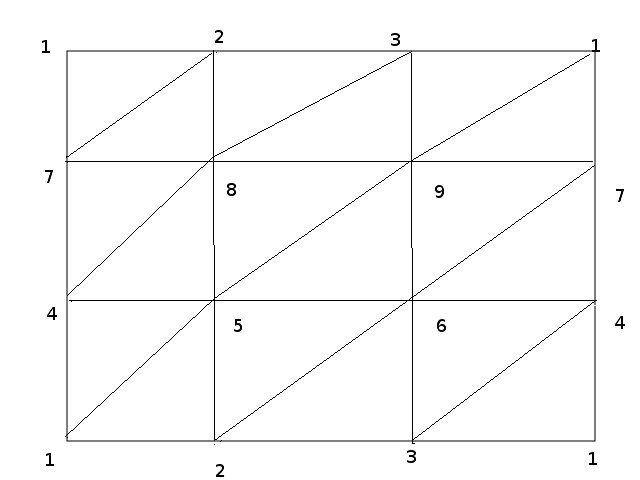
\includegraphics[scale=0.35]{Triangulation.png}
\caption{Primer triangulacije}
\end{center}
\label{triangulacija}
\end{figure}

\subsection{Klasifikacija}


%----------------------------------------------------------------------------------------
%	SECTION 4
%----------------------------------------------------------------------------------------

\section{Rezultati}
Algoritem smo pognali na podanih testnih primerih. Rezultati testov so naslednji:
\begin{enumerate}
\item Klasifikacija triangulacije iz datoteke SyrfaceK.txt \\
	Podana ploskev je 2 projektivnih ravnin s/z 0 luknjami
\item Klasifikacija triangulacije iz datoteke space\_stationSurface.txt \\
	Podana sta dva identična trikotnika: Trikotnik: (6366, 6367, 6368) in Trikotnik: (6368, 6367, 6366). Podan vhod ni ploskev.
\item Klasifikacija triangulacije iz datoteke space\_stationSurface\_no\_duplicates.txt \\
	Triangulacija ima več komponent! \\
	Podana triangulacija ne predstavlja ploskve
\item Klasifikacija triangulacije iz datoteke disc.txt \\
	Podana ploskev je sfera s/z 1 luknjami
\item Klasifikacija triangulacije iz datoteke SurfaceT.txt \\
	Podana ploskev je 1 torusov s/z 0 luknjami
\item Klasifikacija triangulacije iz datoteke SurfaceGJ1.txt \\
	Podana ploskev je 1 torusov s/z 0 luknjami
\item Klasifikacija triangulacije iz datoteke SurfaceGJ2.txt
	Podana ploskev je 2 projektivnih ravnin s/z 0 luknjami
\end{enumerate}

%----------------------------------------------------------------------------------------
%	SECTION 5
%----------------------------------------------------------------------------------------

\section{Zaključek}

The accepted value (periodic table) is \SI{24.3}{\gram\per\mole} \cite{Smith:2012qr}. The percentage discrepancy between the accepted value and the result obtained here is 1.3\%. Because only a single measurement was made, it is not possible to calculate an estimated standard deviation.

The most obvious source of experimental uncertainty is the limited precision of the balance. Other potential sources of experimental uncertainty are: the reaction might not be complete; if not enough time was allowed for total oxidation, less than complete oxidation of the magnesium might have, in part, reacted with nitrogen in the air (incorrect reaction); the magnesium oxide might have absorbed water from the air, and thus weigh ``too much." Because the result obtained is close to the accepted value it is possible that some of these experimental uncertainties have fortuitously cancelled one another.

%----------------------------------------------------------------------------------------
%	BIBLIOGRAPHY
%----------------------------------------------------------------------------------------

\bibliographystyle{apalike}

\bibliography{sample}

%----------------------------------------------------------------------------------------


\end{document}